 % This file is public domain.

\documentclass[12pt]{article}

\usepackage{graphicx}
\usepackage{color}
\usepackage{flowfram}
\usepackage[a4paper,margin=20mm]{geometry}

\newlength\leftX
\newlength\leftY
\newlength\leftH
\newlength\leftW

\newlength\rightX
\newlength\rightY
\newlength\rightH
\newlength\rightW

\setlength{\leftH}{3cm}
\setlength{\leftY}{\textheight}
\addtolength{\leftY}{-\leftH}

\newstaticframe[1]{\textwidth}{\leftH}{0pt}{\leftY}[title]


\setlength{\leftH}{13cm}
\adjustheight{\leftH}
\addtolength{\leftY}{-\leftH}

\newstaticframe[1]{\textwidth}{\leftH}{0pt}{\leftY}[L]
\setstaticframe*{L}{shape={\parshape=24
0pt 0.5\linewidth
0pt 0.5\linewidth
0pt 0.5\linewidth
0pt 0.5\linewidth
0pt 0.5\linewidth
0pt 0.5\linewidth
0pt 0.5\linewidth
0pt 0.5\linewidth
0pt 0.5\linewidth
0pt 0.5\linewidth
0pt 0.5\linewidth
0pt 0.5\linewidth
0pt 0.5\linewidth
0pt 0.5\linewidth
0pt 0.5\linewidth
0pt 0.5\linewidth
0pt 0.5\linewidth
0pt \linewidth
0pt \linewidth
0pt \linewidth
0pt \linewidth
0pt \linewidth
0pt \linewidth
0pt \linewidth
}}


\addtolength{\rightY}{\leftY}
\addtolength{\rightY}{73mm}
\setlength{\rightW}{0.9in}
\setlength{\rightH}{1.5in}
\setlength{\rightX}{\textwidth}
\addtolength{\rightX}{-\rightW}
\newstaticframe[1]{\rightW}{\rightH}{\rightX}{\rightY}[egg]

\setstaticcontents*{egg}{
\includegraphics[scale=0.9]{egg}}


\setlength{\rightX}{0.5\textwidth}
\addtolength{\rightX}{\columnsep}
\setlength{\rightW}{\textwidth}
\addtolength{\rightW}{-\rightX}
\setlength{\rightY}{\leftY}
\addtolength{\rightY}{2.8cm}
\setlength{\rightH}{\leftH}
\addtolength{\rightH}{-2.8cm}

\newstaticframe[1]{\rightW}{\rightH}{\rightX}{\rightY}[right]

\setstaticframe*{right}{shape={\parshape=15
0pt \linewidth
0pt \linewidth
0pt \linewidth
0pt 0.75\linewidth
0pt 0.65\linewidth
0pt 0.75\linewidth
0pt 0.8\linewidth
0pt 0.8\linewidth
0pt \linewidth
0pt \linewidth
0pt \linewidth
0pt \linewidth
0pt \linewidth
0pt \linewidth
0pt \linewidth
}}

\addtolength{\rightX}{-0.5\columnsep}
\newstaticframe[1]{0pt}{\rightH}{\rightX}{\rightY}[Lrule]
\setstaticcontents*{Lrule}{\makebox[0pt][l]{%
\rule{\columnseprule}{\rightH}\rule{\rightW}{\columnseprule}}}


\setlength{\leftH}{2cm}
\addtolength{\leftY}{-\leftH}

\newstaticframe[1]{\textwidth}{\leftH}{0pt}{\leftY}[midhead]

\inserthrule*{static}{L}{static}{midhead}

\twocolumninarea{\textwidth}{\leftY}{0pt}{0pt}


\newstaticframe[1]{1.6in}{1.6in}{0pt}{0pt}[sheep]

\setstaticcontents*{sheep}{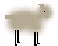
\includegraphics[scale=1.2]{sheep}}

\setcounter{secnumdepth}{0}
\setlength{\sdfparindent}{\parindent}

\begin{document}
\begin{staticcontents*}{title}
\begin{center}
\bfseries\Huge
Fairy Tale Times
\end{center}
\hfill Issue 2. 7 December 2005.
\end{staticcontents*}

\begin{staticcontents*}{L}
\section{Killer Wolf on the Loose}

The authorites are warning of a killer wolf on the
loose. He has so far devoured an old grandmother and
two pig brothers. He is described as being furry with
big eyes and big teeth.

On Monday this week he broke into a house, and devoured
an old lady. He then disguised himself as the old lady
in order to deceive her granddaughter. Luckily for the little
girl a woodsman arrived in time to rescue her. Parents are
being cautioned not to let their children wander about on
their own, and to remind them not to talk to strangers.

The next day the wolf struck again, this time targeting two
pig brothers who had most incautiously made their dwellings
on the cheap using inadequate materials. The wolf also made
an attempt on the third pig brother, but was unable to break
into his house.

Police are appealing to the public for witnesses and remind
people to keep their doors securely fastened at all times.
``Always ask to see identification,'' said one police advisor,
``and invest in improving the general security of your property.''
\end{staticcontents*}

\begin{staticcontents*}{right}
\section{Tragic Wall Accident}

An egg person tragically fell from a six foot wall yesterday
afternoon and was smash\-ed to pieces. The king's cavalry rushed
to the scene, but regretted that they  were unable to help him.

Humpty Dumpty was believed to be sitting on the wall when he fell. Police have ruled out foul play, but
are advising people not to play on high walls, particularly
those vulnerable members of the population suffering from
eggshell syndrome.

\small\em
Exclusive interview with one of the King's men on page 6
\end{staticcontents*}

\begin{staticcontents*}{midhead}
\section{Relief as Missing Sheep Finally Return Home}
\end{staticcontents*}

There was much celebration yesterday morning when Little Bo
Peep's sheep finally returned home. They had been missing
for more than a week.

``I just didn't know where to find them,'' the shepherdess
stated, ``but I was told to leave them alone and they'd come
home.''

\parshape=8
0pt \linewidth
0pt \linewidth
0.3\linewidth 0.7\linewidth
0.3\linewidth 0.7\linewidth
0.25\linewidth 0.75\linewidth
0.25\linewidth 0.75\linewidth
0pt \linewidth
0pt \linewidth
Unusual advice perhaps, but it seems to have worked
as they did indeed come home. Eye witnesses reported that their
tails were wagging behind them.
``I'm just so happy they've come home,'' Little Bo Peep said
in a press conference yesterday afternoon.
The sheep themselves made no comment, and police are%
\framebreak\parshape=0
still trying to determine what happened to them.
The big bad wolf is reportedly helping them with their inquiries.

\noindent\hrulefill

This is a sample document illustrating the
flowfram package. It uses \TeX's \verb|\parshape| command
to create irregularly shaped paragraphs. This can be a complicated
and somewhat tiresome task, and is generally not recommended.
Using the shapepar package provides you with more intricate
shapes, but as its documentation says, it is not intended
for use in large documents.

\hfill Nicola Talbot
\end{document}
